%%=============================================================================
%% Onderzoek
%%=============================================================================

\chapter{\IfLanguageName{dutch}{Onderzoek}{Study}}
\label{ch:onderzoek}



In this study there will be a comparison between the GNFS algorithm on a classical computer and Shor's algorithm on a quantum computer.
In section \ref{sec:Other algorithms} discussing some other algorithms that can show benefits of quantum computing in the industry. To conclude there will be looked into the prime industries it could be used in.

\section{The comparison}
\subsection{General Number Field Sieve}
\subsection{Shor's algorithm}
\subsubsection{Gates}
\label{subsubsec:gates}
For building circuits, this study will be using IBM's quantum composer. The composer can be used in two differnt ways: drag and drop or writing code.
As mentioned in section \ref{sec:Composer} writing code in the composer is done with OpenQASM2.0 and the drag and drop uses lines that represent qubits on which gates or operators can be placed.
Before making the algorithm, first the gates have to be illustrated. All the information of the operations can be found on the webside of IBM \footnote{$https://quantum-computing.ibm.com/composer/docs/iqx/operations_glossary$} on quantum computing as well as in \textcite{Hidary_2019} section 3.1 Quantum operators.
There are 5 types of gates: classicals, quantums, phases, non-unitaries and the Hadamard. Each of these are reversible: when the same operation is used twice on a qubit, it's state will be the same as the starting state \autocite{reversible_gates, revgates}.

The first gates that will be discussed are the classical gates, also known as Pauli gates. In this group 4 gates can be found: the NOT gate, the CNOT gate, the Toffoli gate and the SWAP gate.
In figure \ref{fig:classical gates} the representation of the classical gates in composer is given in the following order, NOT, CNOT, Toffoli and SWAP.
The not gate, or Pauli X gate, flips the state of a qubit. The controlled not gate, or CX, uses 2 qubits. One qubit is the target that will be flipped if the controll qubit is in state $\ket{1}$. It can also function as an operation to make an entanglement.
In this case if the controll qubit is in a superposition, both qubits will be entangled. The Toffoli gate acts as a double CNOT gate. It uses two controll qubits that have to be in the $\ket{1}$ state to flip the target.
Lastly there is the SWAP gate. This is a bit self-explanatory because it just swaps the states of two qubits. There is a special gate called the identity gate. In fact it's not a gate at all, this 'gate' is a blnak unit in th egate time to ensure nothing can happen with that qubit.

\begin{figure} [h]
    \centering
    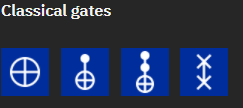
\includegraphics[width=\textwidth]{img/classical-gates.PNG}
        \caption{A visual representation of the classical gates}
        \label{fig:classical gates}
\end{figure}

Next up are the phase gates. This group of gates exists of the T gate, S gate, Z gate, T$\dagger$ gate, S$\dagger$ gate, phase gate and the RZ gate. These gates shift the phase of the qubits.
The T$\dagger$ and S$\dagger$ gates are the inverse gates of the respectively T and S gate. And terh T, S and Z gate are just 'special' cases of the phase gate.
In table \ref{tab:gates} all the shift of the phase for every gates are showed in matrixform.

\begin{table}[]
\label{tab:gates}
    \begin{tabular}{l|l}
    \hline
    \multicolumn{1}{|l|}{Phase Gate}  & \multicolumn{1}{l|}{Shift on the phase}                            \\ \hline
    T                                 & $\begin{pmatrix}1&0// 0& \exp(i\frac{\theta}{4})\end{pmatrix}$     \\
    Z                                 & $\begin{pmatrix}1&0//0& -1\end{pmatrix}$                           \\
    S                                 & $\begin{pmatrix}1&0//0& i\end{pmatrix}$                            \\
    T$\dagger$                        & $\begin{pmatrix}1&0//0& \exp(-i\frac{\theta}{4})\end{pmatrix}$     \\
    S$\dagger $                       & $\begin{pmatrix}1&0//0& -i\end{pmatrix}$                           \\
    P                                 & $\begin{pmatrix}1&0//0& \exp(i\lambda)\end{pmatrix}$               \\
    RZ                                & $\begin{pmatrix}\exp(-i\frac{\lambda}{2})&0//0& \exp(i\frac{\lambda}{2})\end{pmatrix}$                                    
    \end{tabular}
    \caption{The shifts on the phase from any phase gate.}
\end{table}

\begin{figure} [h]
    \centering
    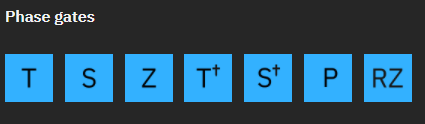
\includegraphics[width=\textwidth]{img/phase-gates.PNG}
        \caption{A visual representation of the phase gates}
        \label{fig:phase gates}
\end{figure}

There are 5 different non-unitary operators or modifiers. These operators are reset, measurement, IF and the barrier operation. There is also one modifier: the control modifier.
The reset operations resets the qubit to the $\ket{0}$. This operation doesn't take any previous state into consideration and is not reversible.
The measurement operation also is not reversible and measures the qubit. So it's output gives the value of the qubit in the standard basis.
Applying an IF operation can give conditions to quantum gates. The conditions in the if operations depend on the state of the classical register, not the quantum one.
When a circuit is executed the computer will try to combine gates to increase te efficiency. If these combinations should not happen, de barrier operation can be used.
Lastly the control modifier is used with another operation. Say for example the Z-gate is used and a control modifier is applied to that, the Z-gate will only be executed if the qubit on which the control lays is in state $\ket{1}$.

\begin{figure} [h]
    \centering
    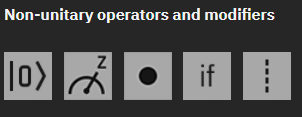
\includegraphics[width=\textwidth]{img/non-unitary-gates.PNG}
        \caption{A visual representation of the non-unitary gates}
        \label{fig:non-uni gates}
\end{figure}

The Hadamard gate is used to make superpositions. When appling this gate to a qubit in state $\ket{1}$ or $\ket{0}$, it rotates it resulting respective states $\ket{-}$ and $\ket{+S}$

\begin{figure} [h]
    \centering
    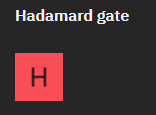
\includegraphics[width=\textwidth]{img/hadamard-gate.PNG}
        \caption{A visual representation of the hadamard gate}
        \label{fig:hadamard gates}
\end{figure}

$\sqrt{x}$, $\sqrt{x}$$\dagger$, Y, RX, RY, RXX, RZZ and U make up the last set of gates: the quantum gates.

\begin{figure} [h]
    \centering
    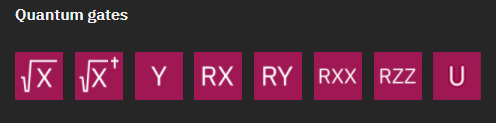
\includegraphics[width=\textwidth]{img/quantum-gates.PNG}
        \caption{A visual representation of the quantum gates}
        \label{fig:quantum gates}
\end{figure}

\section{Other algorithms}
\label{sec:Other algorithms}
\section{The use of quantum computing}